\documentclass[12pt]{article}
\usepackage[top=1in, bottom=1in, left=1in, right=1in]{geometry}

\usepackage{setspace}
\onehalfspacing

\usepackage{amssymb}
%% The amsthm package provides extended theorem environments
\usepackage{amsthm}
\usepackage{epsfig}
\usepackage{times}
\renewcommand{\ttdefault}{cmtt}
\usepackage{amsmath}
\usepackage{graphicx} % for graphics files

% Draw figures yourself
\usepackage{tikz} 

% writing elements
\usepackage{mhchem}

% The float package HAS to load before hyperref
\usepackage{float} % for psuedocode formatting
\usepackage{xspace}

% from Denovo Methods Manual
\usepackage{mathrsfs}
\usepackage[mathcal]{euscript}
\usepackage{color}
\usepackage{array}

\usepackage[pdftex]{hyperref}
\usepackage[parfill]{parskip}

% math syntax
\newcommand{\nth}{n\ensuremath{^{\text{th}}} }
\newcommand{\ve}[1]{\ensuremath{\mathbf{#1}}}
\newcommand{\Macro}{\ensuremath{\Sigma}}
\newcommand{\rvec}{\ensuremath{\vec{r}}}
\newcommand{\omvec}{\ensuremath{\hat{\Omega}}}
\newcommand{\vOmega}{\ensuremath{\hat{\Omega}}}
%---------------------------------------------------------------------------
%---------------------------------------------------------------------------
\begin{document}
\begin{center}
{\bf NE 255, Fa16 \\
Nuclear Physics Basics and Terms\\
August 30, 2016}
\end{center}

\setlength{\unitlength}{1in}
\begin{picture}(6,.1) 
\put(0,0) {\line(1,0){6.25}}         
\end{picture}

A primary goal of nuclear reactor analysis and design is the reliable prediction of neutron population production and loss rates. 
In order to fully describe neutron transport through media, we need to describe neutron motion and neutron interactions with matter.

To begin determining probabilities of neutron-nuclear reactions, we will first review the aspects of nuclear physics that are relevant for fission chain reactions. 

\subsection*{Nuclear Physics of Chain Reactions}
Notation reminder: \ce{^{A}_{Z}X} indicates that chemical element $X$ has $Z$ protons (atomic number) and $A$ total nucleons (protons + neutrons; mass number).\\
Note that this leaves $N$ neutrons.\\
Excited states are written as \ce{^{A}_{Z}X^*}, and metastable/isomeric as \ce{^{A}_{Z}X^m}.

There are two types of \textbf{basic nuclear transformations}
\begin{enumerate}
\item spontaneous disintegration: The spontaneous decay of unstable nuclei, with emission of particles or radiation
\[X \rightarrow Y + y + Q\]
These are probabilistic events that depend only on the type of nucleus.

\item induced by collision: An event in which, because of interaction with a particle or radiation (a projectile), a nucleus (target) is changed in mass, charge or energy state, and particles or radiation is
emitted.
\[x + X \rightarrow Y + y + Q\]
\end{enumerate}
here $y$ and $x$ are typically $\alpha$, $\beta$, or $\gamma$ and $Q$ is energy.

\underline{Examples} of common reactions:
\begin{itemize}
\item Potential elastic scattering $(n,n)$: \ce{^1_0 n} + \ce{^A_Z X} $\rightarrow$ \ce{^1_0 n} + \ce{^A_Z X}

\item Resonance elastic scattering $(n,n)$: \ce{^1_0 n} + \ce{^A_Z X} $\rightarrow$ (\ce{^A_Z X$^*$}) $\rightarrow$ \ce{^1_0 n} + \ce{^A_Z X}

\item Inelastic scattering $(n,n')$: \ce{^1_0 n} + \ce{^A_Z X} $\rightarrow$ (\ce{^A_Z X$^*$}) $\rightarrow$ \ce{^1_0 n} + \ce{^A_Z X} + $\gamma$

\item Radiative capture (absorption) $(n,\gamma)$: \ce{^1_0 n} + \ce{^A_Z X} $\rightarrow$ (\ce{^A_Z X$^*$}) $\rightarrow$ \ce{^A_Z X} + $\gamma$

\item Fission (absorption) $(n,f)$: $(n,\gamma)$: \ce{^1_0 n} + \ce{^A_Z X} $\rightarrow$ \ce{^{A1}_{Z1} X} + \ce{^{A2}_{Z2} X} + (a few)\ce{^1_0 n}

\item Charged-Particle Reactions (absorption): $(n,\alpha)$ \ce{^1_0 n} + \ce{^A_Z X} $\rightarrow$ \ce{^{A-3}_{Z-2} Y} + \ce{^{4}_{2} He}; \\
\hspace*{17 em}$(n,p)$  \ce{^1_0 n} + \ce{^A_Z X} $\rightarrow$ \ce{^{A}_{Z-1} Y} + \ce{^1_1 p}

\item Neutron-Producing Reactions (absorption): $(n,2n)$	 \ce{^1_0 n} + \ce{^A_Z X} $\rightarrow$ \ce{^{A-1}_{Z} X} + 2\ce{^1_0 n}
\end{itemize}

Which reaction happens depends on the type of nucleus, the energy of the incoming neutron, and statistics. We can, fortunately, draw general categories for many types of reactions:

\begin{figure}[h!]
    \begin{center}
    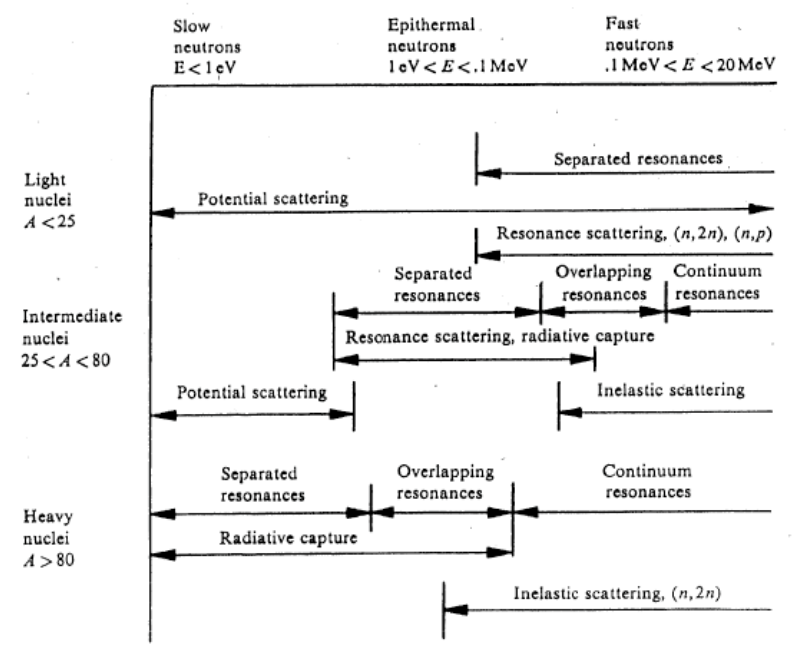
\includegraphics[keepaspectratio, width = 5 in]{reactionenergy}
    \caption{Neutron Interactions by Energy and Atomic Number}
    \label{fig:phase_space}
    \end{center}
\end{figure}

Nuclear Reactions have to obey a set of \textbf{Conservation Laws}, which govern what actually happens in the transformations. 

\begin{itemize}
\item Conservation of Mass/Energy: The total energy of the system before nuclear transformation must be equal to the total energy of the system after the transformation.

\item Conservation of Linear Momentum: Total linear momentum of the system (a vector) before nuclear transformation must be equal to the total linear momentum of the system (a vector) after the transformation.

\item Conservation of Charge: Total charge of the system before nuclear
transformation must be equal to the total charge of the system after the transformation.

\item Conservation of Nucleons: Total number of nucleons (protons and neutrons) of the system before nuclear transformation must be equal to the total number of nucleons (protons and neutrons) of the system after the transformation.
\end{itemize}

The conservation laws govern what reactions can happen. What reactions actually happen govern the neutron population in a reactor. 

What we'll cover next are the definitions and terms we will use to describe neutrons in six-dimensional phase space: $(x,y,z,\vOmega, E)$.

\subsection*{Definitions}

\begin{figure}[h!]
    \begin{center}
    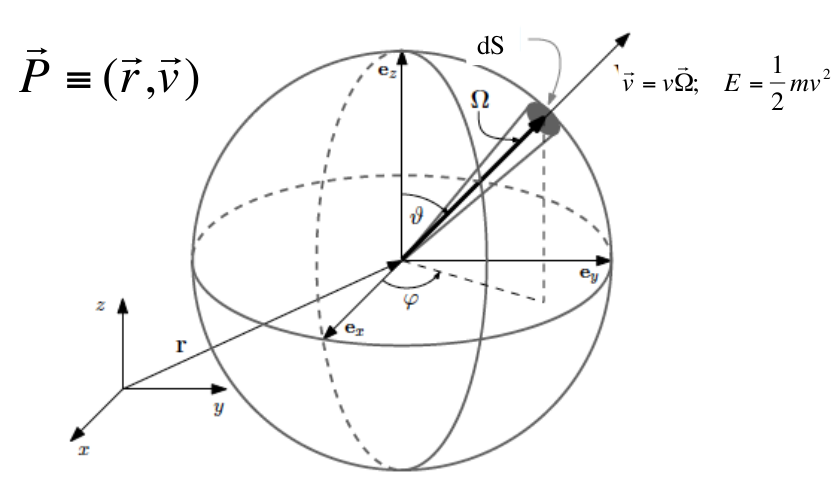
\includegraphics[keepaspectratio, width = 4 in]{phase-space}
    \end{center}
    \caption{Schematic of Phase Space}
    \label{fig:phase_space}
\end{figure}

Spatial logistics
\begin{itemize}
\item $d\vec{r} = d^3r$ = ordinary volume = $r^2 \sin(\theta) d\theta d\varphi dr$
%
\item $v$ = speed (scaler)
\item $\vec{v}$ = $v\vOmega$ = velocity (vector)
\item $d\vec{v} = d^3v$ = velocity volume = $v^2 \sin(\theta)d\theta d\varphi dr$
\item $v = \sqrt{(2E)/m}$ where $m$ is the rest mass of the particle. Thus, we can relate energy and speed.

\item $\vOmega$: unit directional vector in velocity space, $\vec{v} = v\vOmega$
\item $d\vOmega = \sin(\theta)d\theta d\varphi =  d^2\Omega$
%\item thus $d\vec{v} = v^2 dv d\vOmega$
\end{itemize}

These are the possible reactions we're generally going to worry about:

\hspace*{1em}total (t): all interactions. We can break total into:
\begin{itemize}
\item scattering (s): a neutron interacts with an atom and bounces off either elastically or inelastically.
\item absorption (a): a neutron is absorbed by a nucleus. If this happens it might
\item fission (f): cause the nucleus to split into two pieces, releasing more neutrons.
\end{itemize}

Physics terms we will use:
\begin{enumerate}
\item \textbf{microscopic x-sec} ($\sigma$, [$cm^2$]): measure of the probability that an incident neutron will collide with a specific nucleus; $\sigma_j$ indicates a specific reaction, e.g.\ $j=f$ is fission.

\item \textbf{macroscopic x-sec} ($\Sigma$ [$cm^{-1}$]): measure of the probability per unit path length that an incident neutron will collide with a target
\[\Sigma_j = \sigma_j N\:,\]
where N is the atomic density of the target. The total cross section is simply the sum of all possible reaction types, $j$. 

If a material is made of multiple isotopes, the material macroscopic cross section is also the sum over all materials, $i$:
\[
\Sigma_i(\vec{r}, E, t) = \sum_{j=1}^J  N_j(\vec{r}, t)\sigma_{i,j}(E)
\qquad
\Sigma_t(\vec{r}, E, t) = \sum_{j=1}^J \sum_{i=1}^I N_j(\vec{r}, t)\sigma_{i,j}(E)
\]

\item \textbf{double-differential scattering x-sec} ($\sigma_s(E, \vOmega \rightarrow E', \vOmega')dE' d\vOmega'$): measure of the probability that a neutron of energy $E$ and moving in direction $\vOmega$ scatters off of a specific nucleus into energy range $[E', E' + dE']$ and direction range $[\vOmega', \vOmega' + d\vOmega']$.

We can think of this as the fractional probability multiplied by the total scattering cross section
\begin{align*}
\sigma_s(E, \vOmega \rightarrow E', \vOmega') &= \sigma_s(E) f_s(E, \vOmega \rightarrow E', \vOmega')\\
\text{where } &\int_0^{E_0} dE' \int_{4 \pi} d\vOmega' \: f_s(E, \vOmega \rightarrow E', \vOmega') = 1\\
\sigma_s(E) &= \int_0^{E_0} dE' \int_{4 \pi} d\vOmega' \:\sigma_s(E, \vOmega \rightarrow E', \vOmega')
\end{align*}

\item \textbf{fission yield} ($\nu(E)$): average \# of neutrons released by a fission induced by a neutron of energy E.

\item \textbf{fission spectrum} ($\chi(E)dE$): average \# of neutrons produced from fission that are born with energy in $[E, E + dE]$. This is normalized such that
\[\int_0^{\infty} \chi(E)dE =1\:.\]


\begin{itemize}
\item U-235: $\chi(E) = 0.453 e^{-1.036E} \sinh(\sqrt{2.29E})$
\item Pu-239: $\chi(E) = 0.6739 \sqrt{E} e^{-E / 1.41}$
\end{itemize}

\item \textbf{particle angular density} ($n(\vec{r}, E, \vOmega, t)d\vec{r} d\vOmega dE$): expected number of particles in volume element $d^3r$ at $\vec{r}$ whose energies are in $[E, E + dE]$ and direction of motion is in $[\vOmega, \vOmega + d\vOmega]$ at time $t$.

Note:
\begin{align*}
n(\vec{r}, E, \vOmega, t) &= \frac{1}{mv}n(\vec{r}, v, \vOmega, t) \\
n(\vec{r}, v, \vOmega, t) &= v^2 n(\vec{r}, \vec{v}, t) \\
n(\vec{r}, \vec{v}, t) &= \frac{m}{v}n(\vec{r}, E, \vOmega, t)
\end{align*}
\begin{figure}[h!]
    \begin{center}
    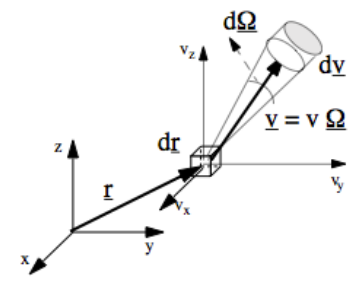
\includegraphics[keepaspectratio, width = 2.5 in]{differential-element}
    \end{center}
    \caption{Differential volume, velocity (energy), and angle}
    \label{fig:phase_space}
\end{figure}

\item \textbf{particle density}: ($N(\vec{r},E,t)d^3r dE$): expected number of particles in $d^3r$ at $\vec{r}$ whose energies are in $[E, E + dE]$ at time $t$.
\[N(\vec{r},E,t)d^3r dE = \int_{4\pi} d\vOmega\: n(\vec{r}, E, \vOmega, t)d^3r dE \]

\item \textbf{angular flux}: $\psi(\vec{r}, E, \vOmega, t) \equiv v n(\vec{r}, E, \vOmega, t)$ [neutrons / (cm$^2$ s MeV steradian)] can be thought of as path length per unit volume about $\vec{r}$ passed by neutrons with energies...

\item \textbf{scalar flux}: $\phi(\vec{r},E,t) \equiv v N(\vec{r},E,t)$ [neutrons / (cm$^2$ s MeV)] can be thought of as the number of neutrons that penetrate a sphere of 1 cm$62$ cross sectional area at $\vec{r}$ with energies in $dE$ about $E$ at time $t$.
%
\[= \int_{4\pi} d\vOmega\: \psi(\vec{r}, E, \vOmega, t) \]

\item \textbf{interaction rate density}: expected number of $j$ reactions per volume per energy at time $t$.
%
\[\int_{4\pi} d\vOmega \:\Sigma_j v n(\vec{r}, E, \vOmega, t) = \Sigma_j \phi(\vec{r},E,t)\]

\item \textbf{angular current density} or partial current: $\vec{j}(\vec{r}, E, \vOmega, t) = \vec{v} n(\vec{r}, E, \vOmega, t)$; 

$\vec{j}(\vec{r}, E, \vOmega, t) \cdot \hat{e}\: dA\: dE\: d\vOmega$ is the expected number of particles crossing $dA$ along unit direction $\hat{e}$ with energy in $[E, E + dE]$ and direction in $[\vOmega, \vOmega + d\vOmega]$ at time $t$.

\item \textbf{net current}: $\vec{J}(\vec{r}, E, t) $ is the net \# of particles crossing a unit area per second along a direction normal to that area with energies in $[E, E + dE]$ at time $t$.
\[\vec{J}(\vec{r}, E, t) = \int_{4\pi} d\vOmega\: \vOmega \psi(\vec{r}, E, \vOmega, t)\]

\end{enumerate}

%-----------------------------------------
\subsection*{Assumptions}
\begin{enumerate}
\item Particles are point objects ($\lambda = h/(mv))$ is small compared to the atomic diameter): its state is fully described by its location, velocity vector, and a given time. This ignores rotation and quantum effects.

\item Neutral particles travel in straight lines between collisions.

\item Particle-particle collisions are negligible (makes TE linear).

\item Material properties are isotropic (generally valid unless velocities are very low).

\item Material composition is time-independent (generally valid over short time scales).

\item Quantities are expected values: fluctuations about the mean for very low densities are not accounted for.
\end{enumerate}

\subsection*{The transport equation}
We consider a six-dimensional volume (as a six-dimensional cube)
 fixed in space, of dimensions
$\triangle x$, $\triangle y$, $\triangle z$, $\triangle E$, $\triangle \theta$, $\triangle \varphi$.
Then, the number of particles within this volume at time $t$ is
\begin{equation*}
n(\rvec,E,\omvec,t)\triangle x\triangle y\triangle z\triangle E\triangle \theta\triangle \varphi =
n(\rvec,E,\omvec,t)\triangle \beta,
\end{equation*}
where all arguments of $N$ are ``average" arguments in the %volume $\triangle V$.
increment of six-dimensional phase space $\triangle \beta$.
The number of
particles in this cube changes with time:
\begin{equation*}
\triangle \beta\frac{\partial}{\partial t}n(\rvec,E,\omvec,t) = \begin{array}{l}
\text{time rate of change of the number of}\vspace{-0.1cm}\\
\text{particles in the six-dimensional cube $\triangle \beta$.}
\end{array}
\end{equation*}
 This time rate of change is due to five separate processes. One is the rate of streaming of
particles out of the volume through the boundaries. The others occur within the
six-dimensional ``cube": the rate
of absorption; the rate of scattering from $E$, $\omvec$ to all other energies and directions, known
as outscattering; the rate of scattering into $E$, $\omvec$ from all other energies and
 directions, known as inscattering; and the rate of production of particles due to an internal source.

 Now, let us consider the surfaces of the cube perpendicular to the $x$-axis. For the net rate
of particles leaving the cube through these two surfaces, we have
\begin{equation*}
(\textrm{Streaming})_x = \dot x n(\rvec,E,\omvec,t)\mid_x^{x+\triangle x}
\triangle y\triangle z\triangle E\triangle \theta \triangle\varphi,
\end{equation*}
 where $\dot x$ is the $x$ component of the particle velocity,
and 
$\triangle y\triangle z\triangle E\triangle\theta\triangle \varphi$ is the surface area. Letting $\triangle x$ go to
the differential $dx$, we rewrite
\begin{equation*}
(\textrm{Streaming})_x = \triangle \beta \frac{\partial}{\partial x}\big[
\dot x n(\rvec,E,\omvec,t)\big].
\end{equation*}
 Using the same procedure for the flow from the cube in the other five ``directions", we obtain
\begin{align*}
\textrm{Streaming} =
\bigg[ \frac{\partial}{\partial x}(\dot x n) + &
\frac{\partial}{\partial y}(\dot y n) +\frac{\partial}{\partial z}(\dot z n) \\
&\quad\quad + \frac{\partial}{\partial E}(\dot E n) + \frac{\partial}{\partial \theta}(\dot \theta n) +
\frac{\partial}{\partial \varphi}(\dot \varphi n)\bigg] \triangle \beta,
\end{align*}
 where $n = n(\rvec,E,\omvec,t)$.


 The rate of absorption within the cube is the product of the number of particles in the cube
and the probability of absorption per particle per unit of time. This probability is given by
the product of the absorption cross section and the particle speed $v$. That is,
\begin{equation*}
\textrm{Absorption} = v\Sigma_a(\rvec,E)n(\rvec ,E,\omvec,t)\triangle \beta.
\end{equation*}
 Using similar arguments and the fact that we need to sum the scattering from (to) $E$,
$\omvec$ to (from) all other energies and directions $E'$, $\omvec'$, we find
\begin{align*}
\textrm{Outscattering} &= \triangle \beta \int_0^{\infty}\int_{4\pi}
v\Sigma_s(\rvec,E\rightarrow E', \omvec\rightarrow\omvec')n(\rvec,E,\omvec,t)d\omvec'dE', \\
\textrm{Inscattering} &= \triangle \beta \int_0^{\infty}\int_{4\pi}
v'\Sigma_s(\rvec,E'\rightarrow E, \omvec'\rightarrow\omvec,)n(\rvec,E',\omvec',t)d\omvec'dE',
\end{align*}
 where $\Sigma_s(\rvec,E'\rightarrow E, \omvec'\rightarrow\omvec)$ is the macroscopic differential scattering cross section. Since the distribution function in the integrand of the outscattering term is independent of
 the integration variables, we can rewrite
Outscattering as $\triangle \beta v\Sigma_s(\rvec,E)n(\rvec, E, \omvec,t).$
Finally, we need to consider the internal source of particles. We
quantify this source  by introducing the function $S(\rvec, E, \omvec, t)$
such that the rate of introduction of particles into the cube is given by
\begin{equation*}
\textrm{Source} = S(\rvec,E,\omvec,t)\triangle \beta.
\end{equation*}

 In order to build the transport equation, we sum these equations with appropriate signs
for loss and gain, to the overall rate of change. Letting $\triangle \beta$ approach a differential
element and canceling it, we obtain
\begin{align}
\frac{\partial n}{\partial t} =& -\left[\frac{\partial (\dot x n)}{\partial x} +
\frac{\partial (\dot y n)}{\partial y}+\frac{\partial (\dot z n)}{\partial z} +
\frac{\partial (\dot E n)}{\partial E}+\frac{\partial (\dot \theta n)}{\partial \theta}+
\frac{\partial (\dot \varphi n)}{\partial \varphi}\right] 
\\ & \quad - v\Sigma_a(\rvec,E)n \nonumber
 \\& \quad\quad\quad   + 
\int_0^{\infty}\int_{4\pi}v'\Sigma_s(\rvec, E'\rightarrow E,\omvec'\rightarrow\omvec)n(\rvec,E',\omvec',t) d\omvec'dE'\nonumber 
\\& \quad\quad\quad\quad\quad\quad -\int_0^{\infty}\int_{4\pi}v\Sigma_s(\rvec, E\rightarrow E',\omvec\rightarrow\omvec')n(\rvec,E,\omvec,t) d\omvec'dE'\nonumber
\\& \quad\quad\quad\quad\quad\quad\quad\quad\quad
+S(\rvec,E,\omvec,t),\nonumber
\end{align}
 where $n = n(\rvec,E,\omvec,t)$. Since particles travel in a straight line
between collisions, \linebreak
$\dot \theta = \dot \varphi = 0$. Furthermore, $\dot E = 0$ because particles stream
with no change in energy. Finally, performing the outscattering integral:
\begin{align}
&\frac{1}{v}\frac{\partial \psi}{\partial t}(\rvec,E,\omvec,t) + \omvec\cdot  \nabla \psi(\rvec,E,\omvec,t) +
 \Sigma_t(\rvec,E)\psi(\rvec,E,\omvec,t)
\\& \quad =
\int_0^{\infty}\int_{4\pi}\Sigma_s(\rvec, E'\rightarrow E,\omvec'\rightarrow\omvec)
\psi(\rvec,E',\omvec',t)d\omvec'dE'+S(\rvec, E, \omvec,t) \nonumber.
\end{align}

We can easily generalize this equation to include nuclear fission.
To do that, we must revisit our treatment of $\Sigma_a$; there are two main processes responsible for the absorption of particles in the system: \textit{radiative capture} and \textit{nuclear fission}. Now, we define
\begin{align*}
\Sigma_\gamma(\rvec,E)ds = \textrm{probability of capture}
\end{align*}
and
\begin{align*}
\Sigma_f(\rvec,E)ds = \textrm{probability of a fission event},
\end{align*}
such that
\begin{align*}
\Sigma_a(\rvec,E) = \Sigma_\gamma(\rvec,E) + \Sigma_f(\rvec,E)\,.
\end{align*}

While a captured neutron is simply removed from the system, a neutron with energy $E$ that induces a fission event causes the target nucleus to split into two smaller daughter nuclei, and 
\begin{align*}
\nu(E) = \textrm{the mean number of fission neutrons that are released}\,.
\end{align*}
Of this number, $\nu(E)[1-M(E)]$ are \textit{prompt} fission neutrons (being emitted within $10^{-15}$ seconds of the fission event). These fission neutrons are emitted isotropically, with an energy distribution given by the fission spectrum $\chi_p(E)$. Also, $\nu(E)M(E)$ \textit{delayed} fission neutrons (being released roughly 0.1 to 60 seconds after the fission event) are created; a delayed neutron is produced when a radioactive daughter nucleus undergoes a radioactive decay process in which a neutron is emitted. 

Assuming (for simplicity) that the number of delayed neutrons emitted by fission is very small [$M(E)<<1$], we can neglect the delayed neutron terms and rewrite
the transport equation as
\begin{align}
&\frac{1}{v}\frac{\partial \psi}{\partial t}(\rvec,E,\omvec,t) + 
\underbrace{\omvec\cdot  \nabla \psi(\rvec,E,\omvec,t)}_{\text{streaming loss rate}} +
 \underbrace{\Sigma_t(\rvec,E)\psi(\rvec,E,\omvec,t) }_{\text{total interaction loss rate}}
\\& \quad\quad\quad\quad =
\underbrace{\int_0^{\infty}\int_{4\pi}\Sigma_s(\rvec, E'\rightarrow E,\omvec'\rightarrow\omvec)
\psi(\rvec,E',\omvec',t)d\omvec'dE'}_{\text{in scattering source rate}}\nonumber
\\&\quad\quad\quad\quad\quad\quad +\underbrace{\frac{\chi_p(E)}{4\pi}\int_0^{\infty}\int_{4\pi}\nu(E')\Sigma_f(\rvec,E')
\psi(\rvec,E',\omvec',t)d\omvec'dE'}_{\text{fission source rate}}\nonumber
\\&\quad\quad\quad\quad\quad\quad\quad\quad+\underbrace{S(\rvec, E, \omvec,t)}_{\text{external source rate}} \nonumber.
\end{align}
   
   
\subsection*{boundary and initial conditions}
These equations require both spatial and temporal boundary conditions.
\textit{Assuming that the
physical
system of interest is nonreentrant} (convex) and characterized by a
volume $V$, it is sufficient to specify the flux of
particles at all points of the bounding surface of the system in the incoming
directions. This implies
\begin{align*}
\psi(\rvec_s, E,\omvec,t) &= \psi_b(\rvec_s,E,\omvec,t)\,, \hspace{0.5 cm} \textbf{n} \cdot \omvec <0,
\end{align*}
 where $\psi_b$ is a specified function at the boundary, $\rvec_s$ is a point on the surface, and $\textbf{n}$ is the unit
outward normal vector at this point. In the time variable, we assume the range of
interest $0\leq t<\infty$ and specify the
initial condition at $t=0$, such that
\begin{align*}
\psi(\rvec,E,\omvec,0) = \psi_0(\rvec,E,\omvec),
\end{align*}
 where $\psi_0$ is a specified function.

A few other boundary conditions that we frequently use in nuclear engineering
\begin{itemize}
\item mirror reflecting: $\psi(\vec{r}, E, \vOmega, t) =  \psi(\vec{r}, E, \vOmega', t) \quad \forall \vec{r} \in S$, where $S$ is a surface, and $\hat(e)\cdot \vOmega < 0$
\item isotropic reflecting: $\psi(\vec{r}, E, \vOmega, t) =  \dfrac{\phi(\vec{r}, E, t)}{4\pi}$
\item vacuum: $\psi(\vec{r}, E, \vOmega, t) = 0\quad \forall \vec{r} \in S$, where $S$ is a surface, and $\hat(e)\cdot \vOmega < 0$ \\
$J^-(\vec{r}, E, t) = \int_{\hat(e)\cdot \vOmega < 0} d\vOmega \: |\hat(e)\cdot \vOmega| \psi(\vec{r}, E, \vOmega, t) = 0$
\item periodic: $\psi(\vec{r}, E, \vOmega, t) = \psi(\vec{r} + d, E, \vOmega, t)$
\end{itemize}

\begin{figure}[h!]
    \begin{center}
    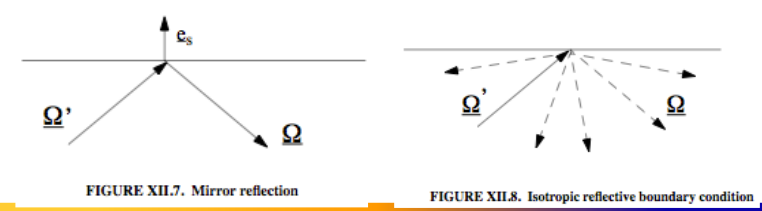
\includegraphics[keepaspectratio, width = 3.5 in]{reflecting-bc}
     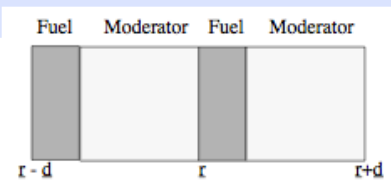
\includegraphics[keepaspectratio, width = 2 in]{periodic-bc}
    \end{center}
\end{figure}

\subsection*{Additional Conditions}
\begin{itemize}
\item Finiteness condition: $0 \leq \psi(\vec{r}, E, \vOmega, t) \leq \infty$
\item Interface condition: $\psi_1(\vec{r}, E, \vOmega, t) = \psi_2(\vec{r}, E, \vOmega, t) \qquad \forall \vec{r} \in S_i$, all energies, and all $\vOmega$
\item Source condition: $Q(\vec{r_0}, E, \vOmega, t) = Q_0(E, \vOmega, t)\delta(\vec{r} - \vec{r_0})$
\end{itemize}

\begin{figure}[h!]
    \begin{center}
    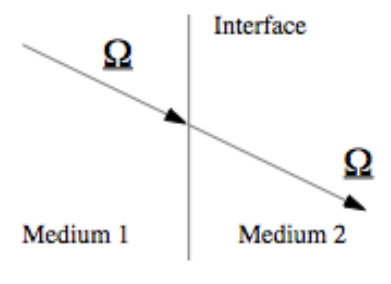
\includegraphics[keepaspectratio, width = 1.5 in]{interface}
     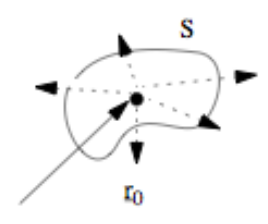
\includegraphics[keepaspectratio, width = 1.5 in]{source}
    \end{center}
\end{figure}

\subsection*{Simplifications} 
It is common to make extra assumptions in order to obtain a simpler version of these equations. For instance, in the case of time-independent, monoenergetic particle transport in a homogeneous medium with a known interior isotropic source:
\begin{align*}
\omvec\cdot  \nabla \psi(\rvec,\omvec) +
 \Sigma_t\psi(\rvec,\omvec)
=
\int_{4\pi}\Sigma_s(\omvec'\rightarrow\omvec)
\psi(\rvec,\omvec')d\omvec'+\frac{S(\rvec)}{4\pi}\,,
\end{align*}
and 
\begin{align*}
\omvec\cdot  \nabla \psi(\rvec,\omvec) +
 \Sigma_t\psi(\rvec,\omvec)%\\&
 &=
\int_{4\pi}\Sigma_s(\omvec'\rightarrow\omvec)
\psi(\rvec,\omvec')d\omvec'\\&\quad\quad\quad\quad\quad\quad
 +\frac{\nu\Sigma_f}{4\pi}\int_{4\pi}
\psi(\rvec,\omvec')d\omvec'+\frac{S(\rvec)}{4\pi}\,.\nonumber
\end{align*}
Both the equations above need a spatial boundary condition, which is given by
\begin{align*}
\psi(\rvec_s,\omvec) = \psi_b(\rvec_s,\omvec)\,, \hspace{0.5 cm} \textbf{n} \cdot \omvec <0\,.
\end{align*}

In steady-state reactor calculations, one often sees a version of these equations in which the inhomogeneous source $S(\rvec)$ and the boundary source $\psi_b(\rvec_s,\omvec)$ are set to zero, and the fission source is modified by a constant factor $1/k$:
\begin{align*}
&\omvec\cdot  \nabla \psi(\rvec,\omvec) +
 \Sigma_t\psi(\rvec,\omvec)%\\&
 =
\int_{4\pi}\Sigma_s(\omvec'\rightarrow\omvec)
\psi(\rvec,\omvec')d\omvec'\\&\quad\quad\quad\quad\quad\quad\quad\quad\quad\quad\quad\quad\quad\quad\quad\quad\quad\quad
 +\frac{\nu\Sigma_f}{4\pi k}\int_{4\pi}
\psi(\rvec,\omvec')d\omvec'\,,\nonumber\\
&\psi(\rvec_s,\omvec) = 0, \hspace{0.5 cm} \textbf{n} \cdot \omvec <0\,.
\end{align*}
These equations always have the zero solution $\psi = 0$; the goal is to find the largest value of $k$ such that a nonzero solution $\psi$ exists. The resulting $k$ is called the \textit{criticality} (or \textit{criticality eigenvalue}) of the system. If a system has a fissile region, it can be shown that $k$ always exists, and the corresponding (eigenfunction) $\psi$ is unique and positive.


\end{document}
